% Security-Gym environment interaction loop (vector schematic).
%
% Build:  pdflatex env-schematic.tex   ->  env-schematic.pdf
%
% Note: the 'standalone' class is preferred for figures like this, but it is
% not present in this minimal TeX Live install. This file instead uses a small
% self-cropping 'article' wrapper (only tikz + graphicx, both available) that
% sizes the PDF page exactly to the figure box plus a 2pt border, so the result
% is an equivalent tightly-cropped vector PDF resized to 5.5in wide. The TikZ
% body below is the actual figure and can be dropped into a 'standalone'
% document unchanged on a fuller TeX install.
\documentclass{article}
\usepackage[T1]{fontenc}
\usepackage{lmodern}
\usepackage{graphicx}
\usepackage{tikz}
\usetikzlibrary{positioning,arrows.meta,backgrounds,fit,calc}

\pagestyle{empty}
\setlength{\parindent}{0pt}
\setlength{\parskip}{0pt}

\begin{document}
\newsavebox{\figbox}
\begin{lrbox}{\figbox}%
\resizebox{5.5in}{!}{%
%================= FIGURE BODY (portable; drop-in for standalone) =================
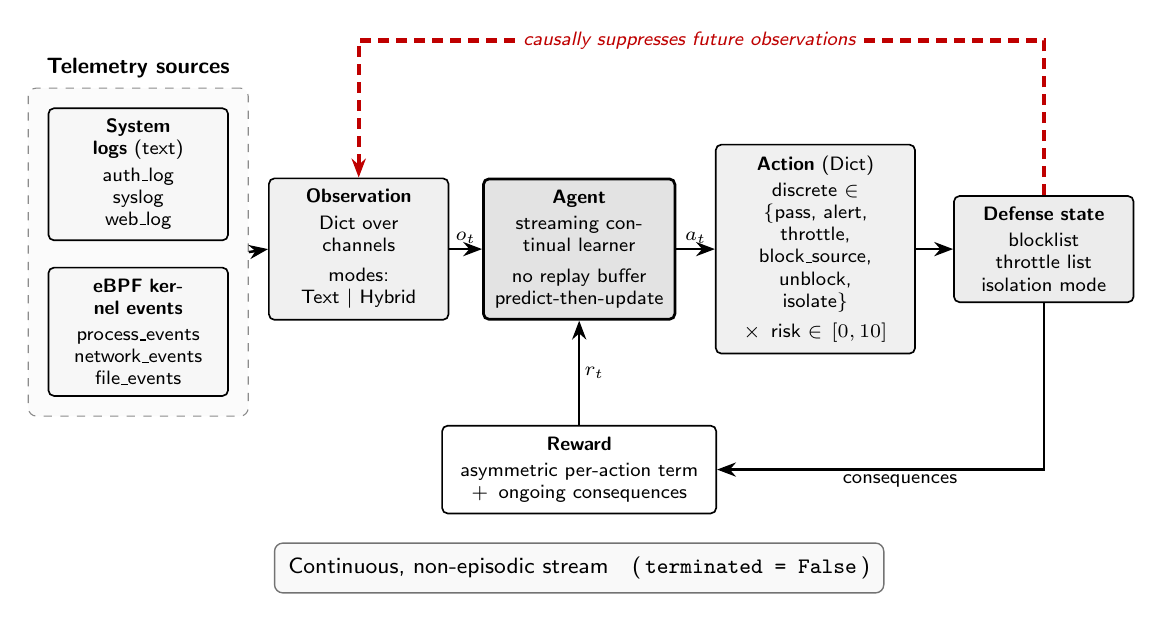
\begin{tikzpicture}[
  >={Stealth[length=2.4mm,width=1.8mm]},
  font=\sffamily,
  nd/.style={draw=black, line width=0.6pt, rounded corners=2pt, align=center,
             inner sep=4pt, font=\scriptsize\sffamily, fill=gray!8},
  flow/.style={->, line width=0.9pt, draw=black},
  lbl/.style={font=\scriptsize\sffamily, inner sep=1.5pt},
  feedback/.style={->, line width=1.5pt, draw=red!75!black, dashed,
                   dash pattern=on 4pt off 2.5pt},
  banner/.style={draw=black!55, line width=0.5pt, rounded corners=3pt,
                 fill=gray!5, align=center, font=\footnotesize\sffamily, inner sep=5pt},
]

% ---------------- telemetry sources (left) ----------------
\node[nd, text width=2.0cm, fill=gray!6] (t1) at (0,0.95)
  {\textbf{System logs} (text)\\[1.5pt] auth\_log\\ syslog\\ web\_log};
\node[nd, text width=2.0cm, fill=gray!6] (t2) at (0,-1.05)
  {\textbf{eBPF kernel events}\\[1.5pt] process\_events\\ network\_events\\ file\_events};

% ---------------- observation ----------------
\node[nd, text width=2.0cm, fill=gray!12] (obs) at (2.8,0)
  {\textbf{Observation}\\[1.5pt] Dict over channels\\[3pt] modes:\\ Text $|$ Hybrid};

% ---------------- agent (focal) ----------------
\node[nd, text width=2.15cm, fill=gray!22, line width=1.0pt] (agent) at (5.6,0)
  {\textbf{Agent}\\[1.5pt] streaming continual learner\\[3pt] no replay buffer\\
   predict-then-update};

% ---------------- action (right) ----------------
\node[nd, text width=2.25cm, fill=gray!12] (act) at (8.6,0)
  {\textbf{Action} (Dict)\\[1.5pt] discrete $\in$\\ \{pass, alert, throttle,\\
   block\_source, unblock,\\ isolate\}\\[3pt] $\times$\, risk $\in [0,10]$};

% ---------------- defense state ----------------
\node[nd, text width=2.0cm, fill=gray!15] (def) at (11.5,0)
  {\textbf{Defense state}\\[1.5pt] blocklist\\ throttle list\\ isolation mode};

% ---------------- reward ----------------
\node[nd, text width=3.2cm, fill=white] (rew) at (5.6,-2.8)
  {\textbf{Reward}\\[1.5pt] asymmetric per-action term \,$+$\, ongoing consequences};

% ---------------- telemetry grouping (background) ----------------
\begin{scope}[on background layer]
  \node[draw=black!45, dashed, rounded corners=3pt, inner sep=7pt, fill=gray!3,
        fit=(t1)(t2),
        label={[font=\footnotesize\sffamily\bfseries]above:Telemetry sources}] (tel) {};
\end{scope}

% ---------------- forward flow ----------------
\draw[flow] (tel.east)   -- (obs.west);
\draw[flow] (obs.east)   -- node[lbl,above]{$o_t$} (agent.west);
\draw[flow] (agent.east) -- node[lbl,above]{$a_t$} (act.west);
\draw[flow] (act.east)   -- (def.west);

% ---------------- reward sub-loop ----------------
\draw[flow] (def.south) |- node[lbl,below,pos=0.72]{consequences} (rew.east);
\draw[flow] (rew.north) -- node[lbl,right]{$r_t$} (agent.south);

% ---------------- critical feedback edge ----------------
\draw[feedback] (def.north) -- (11.5,2.65) -- (2.8,2.65) -- (obs.north);
\node[font=\scriptsize\sffamily\itshape, text=red!75!black,
      fill=white, inner sep=1.5pt] at (7.0,2.65)
      {causally suppresses future observations};

% ---------------- non-episodic banner ----------------
\node[banner] at (5.6,-4.05)
  {Continuous, non-episodic stream\quad(\,\texttt{terminated = False}\,)};

\end{tikzpicture}%
%================= END FIGURE BODY =================
}%
\end{lrbox}%

% Size the PDF page to the figure box plus a uniform 2pt border, then ship a
% single page manually (bypasses the article output routine so no blank page).
\newlength{\bdr}\setlength{\bdr}{2pt}
\pdfpagewidth=\dimexpr\wd\figbox+2\bdr\relax
\pdfpageheight=\dimexpr\ht\figbox+\dp\figbox+2\bdr\relax
% Cancel TeX's default 1in page-origin offset so the shipped box sits flush
% against the page corner (the 2pt border is added by the surrounding box).
\hoffset=-1in
\voffset=-1in
\shipout\vbox{\offinterlineskip
  \vskip\bdr
  \hbox{\hskip\bdr\relax\usebox{\figbox}\hskip\bdr}%
  \vskip\bdr}%
\end{document}
